\section{Vision-Language Models for Document Understanding}
\label{sec:vlm}

Vision-Language Models (VLMs) have propelled visual document understanding from single-modality analysis toward unified multimodal modeling. By jointly modeling visual content, textual semantics, and spatial layout information, VLMs enable deeper understanding of document structures and their semantic relationships. This section traces VLM evolution across four dimensions (\cref{fig:vlm_evolution}): foundational models, high-resolution perception, OCR-free approaches, and agentic systems.

\subsection{Foundational Vision-Language Models}

\subsubsection{Foundational Period of Visually-Rich Document Understanding}

Early research established technical foundations for document image classification and cross-modal retrieval. Deep multimodal learning for cross-modal retrieval \cite{wei2020deep} proposed a ``unified model'' encoding vision and text into the same retrievable representation space.

The pre-training era brought multimodal integration. LayoutXLM \cite{xu2021layoutxlm} introduced multimodal pre-training for multilingual, visually-rich documents. VinVL \cite{zhang2021vinvl} systematically investigated the role of visual features in multimodal tasks. CLIP-Adapter \cite{gao2021clipadapter} proposed efficient adaptation through lightweight feature adapters.

Generalized document processors emerged in 2022. FLAVA \cite{singh2022flava} presented a foundational model using both image-text pairs and unimodal data. UDOP \cite{li2022udop} unified vision, text, and layout as a sequence-to-sequence generative task. Bi-VLDoc \cite{yang2022bivldoc} designed bidirectional vision-language supervision. CM3 \cite{ai2022cm3} adopted causal masked multimodal pre-training for both understanding and generation.

\subsubsection{The Rise of VLM and Advancements in High-Resolution Perception}

LLM integration enabled instruction-driven document understanding. PaLM-E \cite{driess2023palme} proposed an embodied multimodal language model processing various sensor inputs. MiniGPT-4 \cite{zhu2023minigpt4} aligned frozen visual encoders with powerful LLMs through single projection layers. PaLI-X \cite{chen2023palix} scaled multilingual VLMs for document understanding and few-shot learning.

High-resolution processing became a core focus (2023--2024). Monkey \cite{li2024monkey} systematically studied the impact of image resolution and text label quality, noting that resolution improvements often yield more significant gains than structural changes in document scenarios. TextMonkey \cite{li2024textmonkey} proposed an end-to-end OCR-free document understanding model. Qwen2-VL \cite{wang2024qwen2vl} addressed resolution instability through unified modeling supporting arbitrary resolution inputs.

Efficiency and specialization advances included DocKylin \cite{liu2024dockylin} with efficient visual slimming strategies, DocPedia \cite{zhao2023docpedia} exploring frequency-domain information, and Vary \cite{huang2023vary} arguing for visual vocabulary expansion. Small model research \cite{chen2023pali3,li2024slmrvv} achieved strong multimodal understanding at reduced scales.

\begin{figure*}[t]
\centering
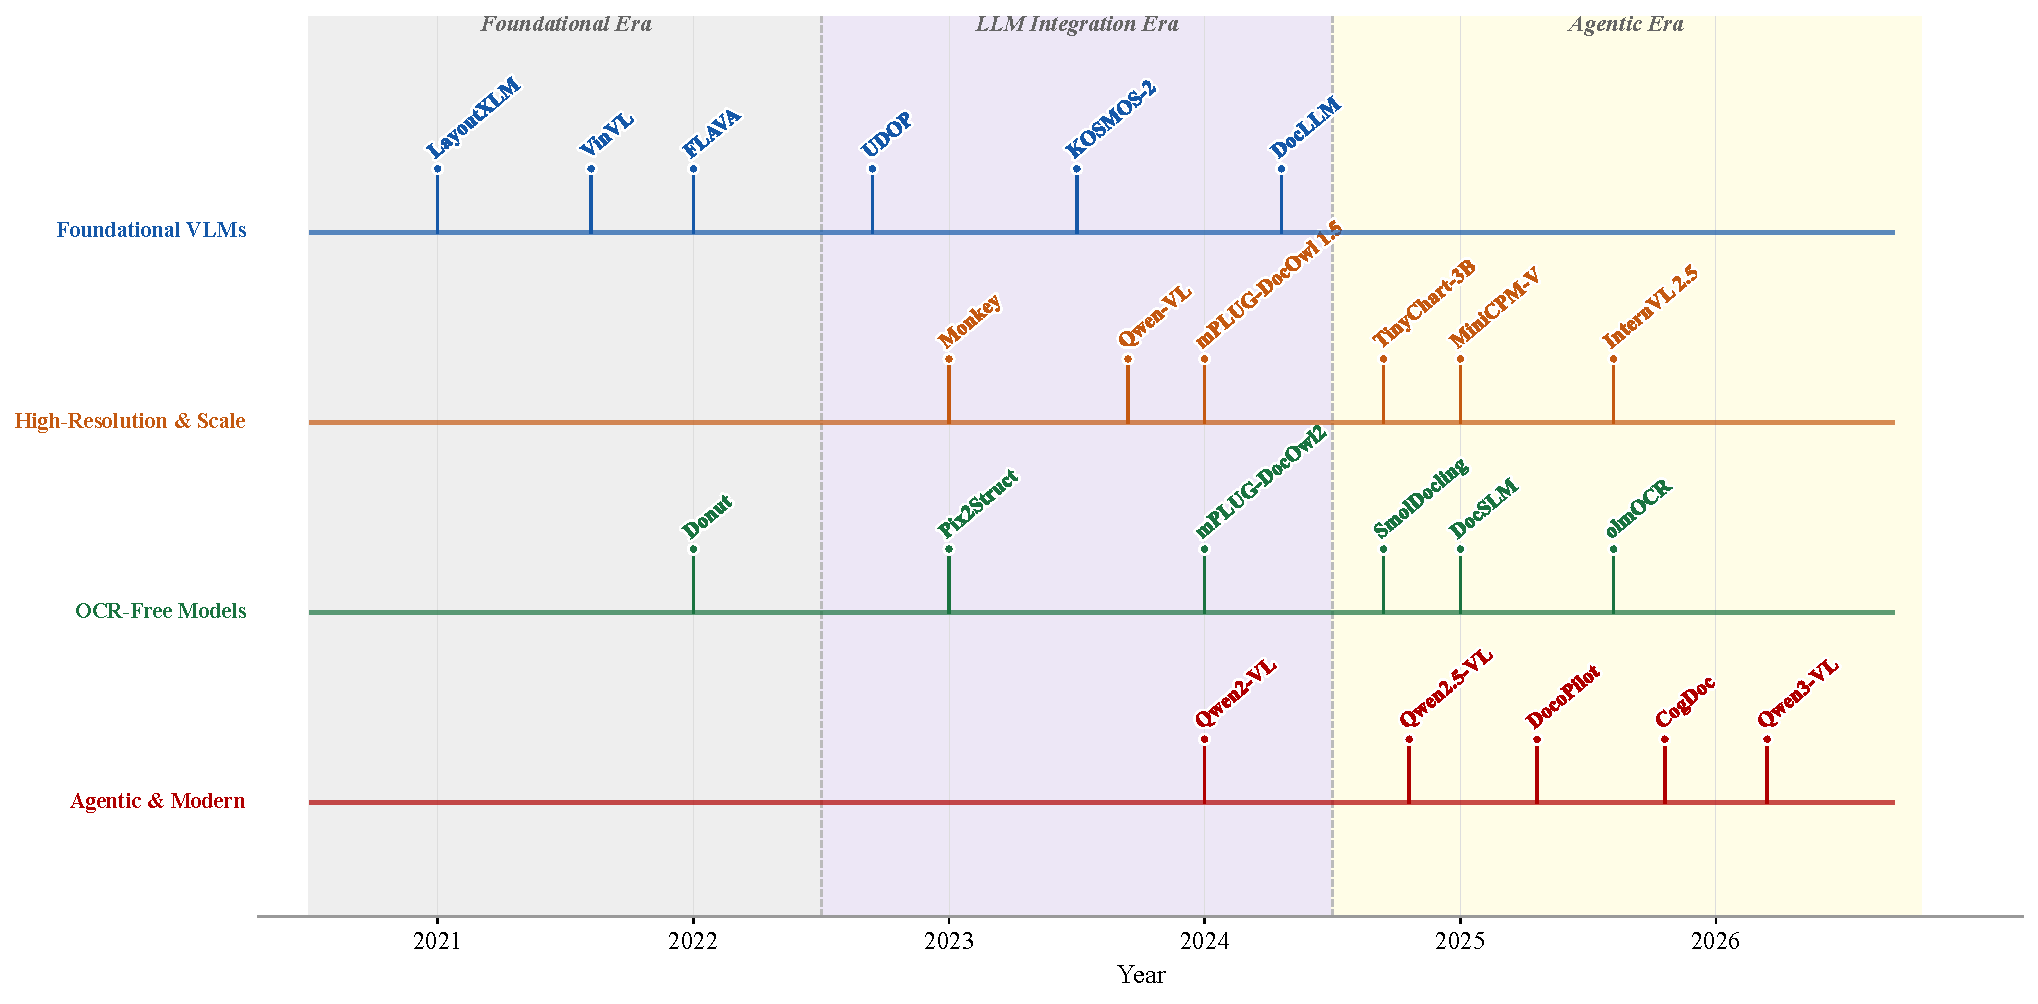
\includegraphics[
    width=0.95\textwidth,
    trim=0cm 0cm 0cm 0cm,
    clip
]{figs/fig07.pdf}
\caption{Evolution of vision-language models for document understanding (2021--2026)---organized into four development tracks: foundational vision-language models, high-resolution and scaled architectures, OCR-free models, and agentic systems for complex document reasoning.}
\label{fig:vlm_evolution}
\end{figure*}

\subsection{OCR-Free and Multi-Page Context}

Traditional document understanding relies on OCR to convert document images into text before semantic analysis, disconnecting ``text recognition'' and ``document understanding'' into independent steps. OCR-free models utilize joint vision-language modeling, taking raw document images as direct input.

Donut \cite{kim2022donut} was an end-to-end document understanding model not relying on OCR systems, generating structured text output directly from raw document images. Pix2Struct \cite{lee2023pix2struct} proposed OCR-free VLM based on screenshot parsing pre-training. mPLUG-DocOwl \cite{ye2023docowl} introduced modularized MLLM for OCR-free document understanding.

Multi-page and long-document capabilities expanded applicability. mPLUG-DocOwl2 \cite{ye2024docowl2} proposed efficient visual compression and structural modeling for multi-page documents. DeepSeek-VL2 \cite{deepseek2024vl2} adopted Mixture-of-Experts architecture for parameter efficiency. PDF-WuKong \cite{li2024pdfwukong} addressed long PDF reading through end-to-end sparse sampling. LongFin \cite{chen2024longfin} introduced models specifically for long financial documents.

Complex document parsing advances included MinerU2.5 \cite{liu2025mineru25} with coarse-to-fine two-stage parsing, and POINTS-Reader \cite{wang2025pointsreader} for distillation-free adaptation. Small VLMs \cite{h2ovl2024mississippi} met privacy-sensitive and on-device scenario needs.

\subsection{Modern Document Understanding Evolution}

The years 2025--2026 witnessed explosive development of ultra-lightweight models. DocSLM \cite{wang2025docslm} addressed computational and memory bottlenecks in long document understanding. SmolDocling \cite{kim2025smoldocling} focused on end-to-end multimodal document conversion through universal DocTags format.

Domain-specific applications expanded. Baseer \cite{albaseer2025baseer} designed specialized VLM for Arabic document OCR. IndoColSmol \cite{rahman2025indocolsmol} targeted multimodal Indonesian document search. Semantic Document Derendering \cite{kim2025derendering} parsed complex documents into editable vector formats.

Document-level strategy research included Docopilot \cite{duan2025docopilot} addressing multi-page document-level tasks, and Nayana \cite{kolavi2025nayana} building multi-task, multimodal, multilingual foundational resources. Qwen2.5-VL \cite{bai2025qwen25vl} and Qwen3-VL \cite{bai2025qwen3vl} established performance benchmarks for unified vision-language understanding.

\subsection{Multimodal RAG}

Building on text RAG success, researchers extended retrieval-augmented paradigms to Visual Document QA, forming early multimodal transitions centered on OCR/structural parsing + text retrieval.

PDF-MVQA \cite{ding2024mvqa} constructed multi-page visually-rich document QA datasets with joint coarse-to-fine retrieval. CREAM \cite{zhang2024cream} introduced coarse-to-fine retrieval pipelines for long contexts. DocLLM \cite{wang2024docllm} mitigated text-layout relationship neglect in traditional VLMs. ViTLP \cite{mao2024visually} jointly modeled text and layout during pre-training.

As ``OCR + text retrieval'' exposed structural and visual information loss, research shifted toward OCR-free visual retrieval. ColPali \cite{faysse2024colpali} proposed page-level OCR-free document retrieval using VLMs for multi-vector page representations, introducing the ViDoRe benchmark. Document Screenshot Embedding \cite{ma2024unifying} used screenshots as unified retrieval input.

Recent multimodal RAG focuses on multi-page, multi-document, multimodal evidence fusion. VisRAG \cite{yu2024visrag} and VDocRAG \cite{tanaka2025vdocrag} pioneered VLM-based retrieval. M3DocRAG \cite{cho2024m3docrag} systematically proposed multi-page, multi-document, multimodal DocQA tasks. CMRAG \cite{chen2025cmrag} mitigated unimodal bias through dual-channel retrieval. RegionRAG \cite{li2025regionrag} lowered retrieval granularity to region level. Luminirag \cite{martis2024luminirag} and MMGraphRAG \cite{wan2025mmgraphrag} unified vision and text into graph structures.

\subsection{Agentic Frameworks for Document QA}

Research has shifted from static RAG to agentic reasoning frameworks with process modeling capabilities.

CuriousLLM \cite{yang2025curiousllm} introduced curiosity-driven follow-up question generation based on Knowledge Graph Prompting, actively guiding retrieval and expanding evidence coverage. DocLens \cite{zhu2025doclens} proposed a tool-enhanced multi-agent framework for long visual document understanding through explicit page-level zooming.

Multi-agent systems improved coordination. MA-RAG \cite{nguyen2025ma} decoupled question decomposition, retrieval control, evidence extraction, and answer synthesis through collaborative chain-of-thought communication. ViDoRAG \cite{wang2025vidorag} proposed dynamic iterative reasoning agents with exploration-reflection workflows.

Research-level complex queries motivated unified systems. Doc-Researcher \cite{dong2025doc} unified multimodal document parsing, dynamic multi-granularity retrieval, and multi-agent reasoning. HEAR \cite{chen2025hear} introduced agentic reasoning into document understanding, establishing coordination between information extraction and reasoning generation. CogDoc \cite{xu2025cogdoc} proposed a unified coarse-to-fine thinking paradigm based on cognitive modeling.

\begin{figure*}[t]
\centering
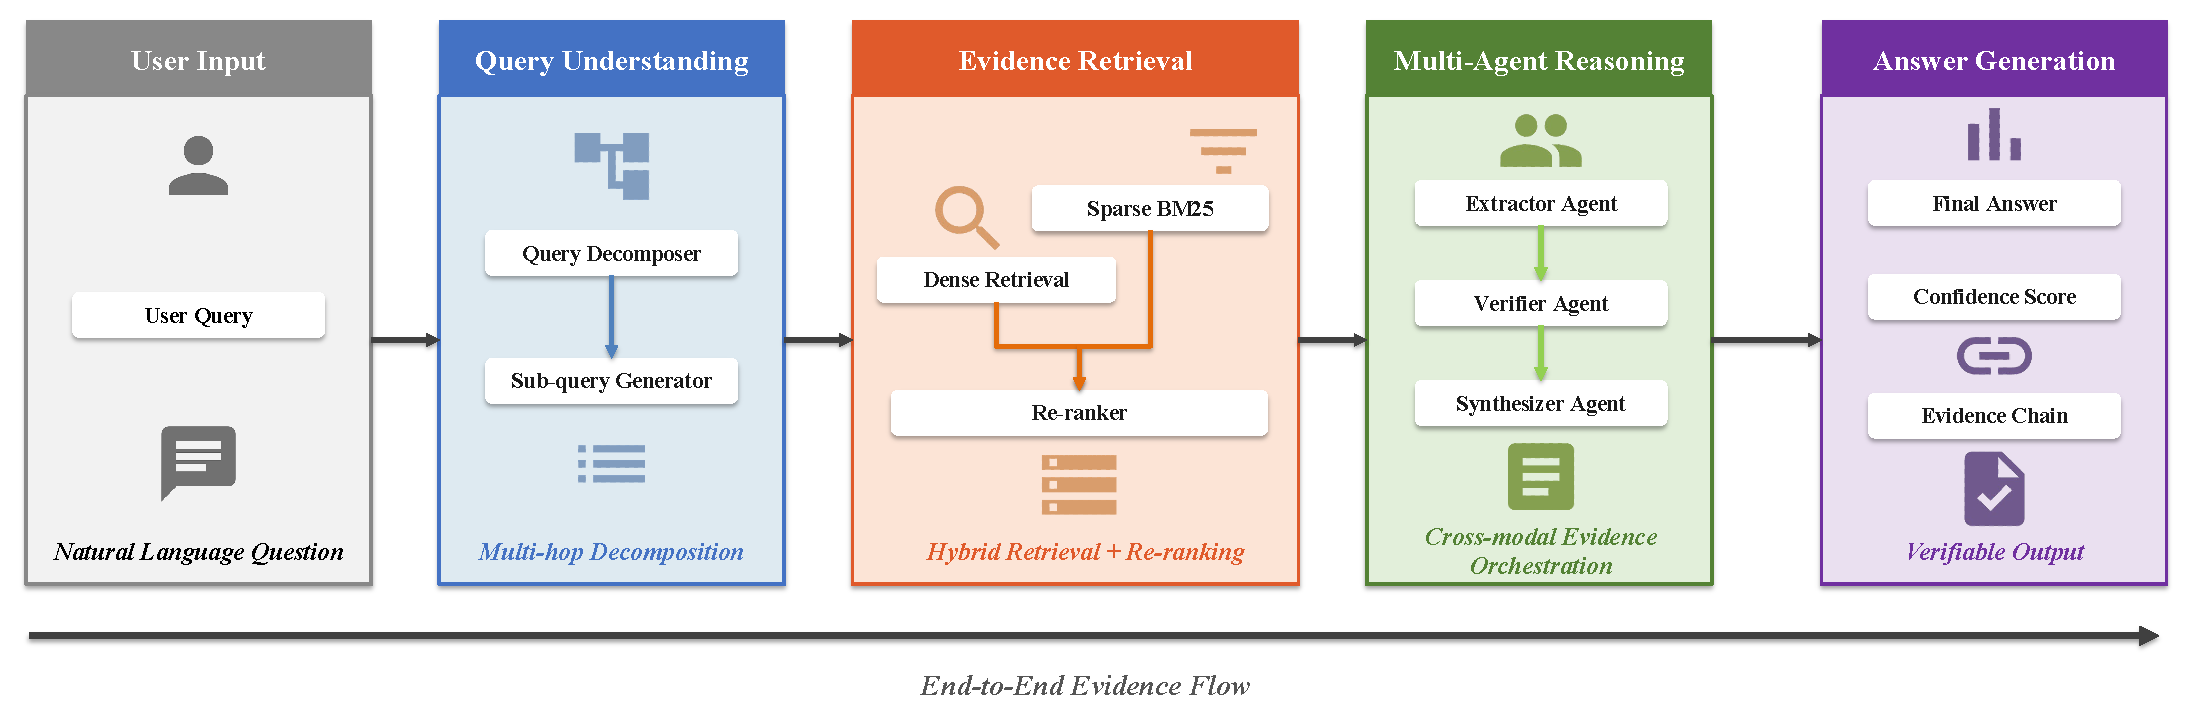
\includegraphics[
    width=0.95\textwidth,
    height=0.40\textheight,
    keepaspectratio,
    trim=0cm 0cm 0cm 0cm,
    clip
]{figs/fig08.pdf}
\caption{Agentic Document QA pipeline illustrating end-to-end evidence flow: a user natural language query passes through Query Understanding (multi-hop decomposition), Evidence Retrieval (hybrid dense and sparse retrieval with re-ranking), Multi-Agent Reasoning (extractor, verifier, and synthesizer agents for cross-modal evidence orchestration), and Answer Generation (producing a final answer with an evidence chain and confidence score).}
\label{fig:agent_docqa}
\end{figure*}
